\subsubsection{Software System}

\paragraph{Communication System} \ \\
\vspace{-0.5cm}
Some communication system talk.


\paragraph{Graphical User Interface} \ \\
Our GUI prioritizes stability, usability, and responsiveness, balancing personalization with default configurations. Built with Python and PyQt5, it ensures a stable and efficient desktop experience.

\vspace{0.2cm}
\textbf{System Architecture}
The GUI follows a modular design, dividing functionality across four interfaces: Pilot, Copilot, Engineer, and Float. This enhances maintainability while tailoring tools to each role.

\vspace{0.2cm}
\textbf{Pilot Interface}
Designed for minimal clutter, the Pilot interface displays five camera feeds essential for navigation. To ensure smooth streaming, we use Python's \texttt{Multiprocessing} library, preventing latency and glitches. The Pilot can switch views and resize feeds as needed. Our redundant streaming system prevents a single point of failure—if one camera disconnects, others remain functional. 

\vspace{0.2cm}
\textbf{Copilot Interface}
The Copilot interface extends camera controls, allowing real-time brightness, contrast, and backlight adjustments for varying underwater conditions. It also displays telemetry data, including six degrees of freedom (Vx, Vy, Vz, Roll, Pitch, Yaw), depth, and thruster speeds, aiding in system monitoring and troubleshooting. A screenshot of the interface is shown in Figure \ref{fig:copilot_interface}.

\begin{figure}[ht]
    \centering
    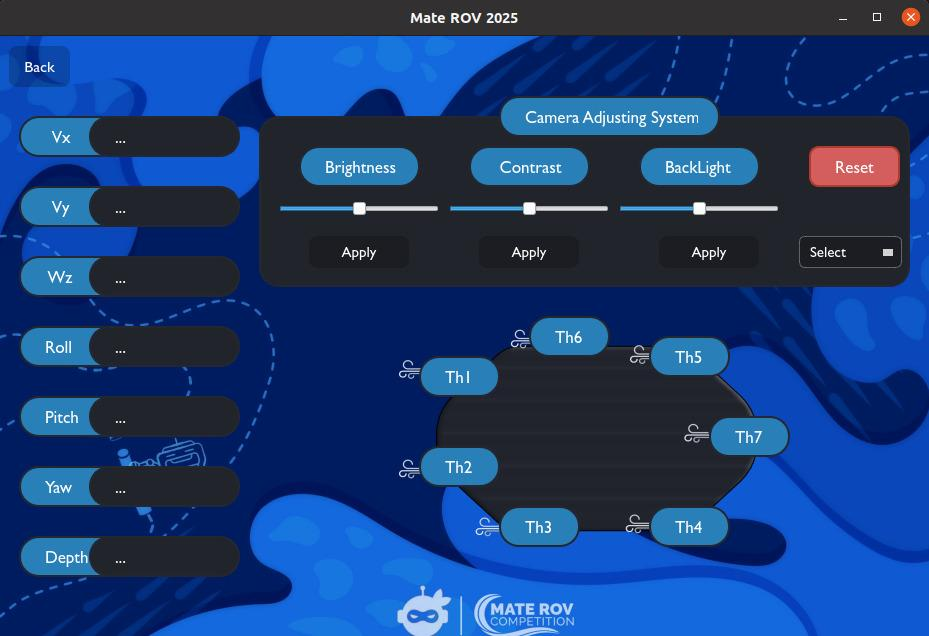
\includegraphics[width=0.8\columnwidth]{Sections/2Design Rationale/images/Copilot_interface.jpeg}
    \caption{Screenshot of the Copilot interface.}
    \label{fig:copilot_interface}
\end{figure}

\vspace{0.2cm}
\textbf{Engineer Interface}
The Engineer interface provides quick access to automation scripts for tasks like invasive carp detection and depth estimation. It also facilitates seamless media capture for Photosphere documentation. All functions are integrated within the GUI, streamlining workflow without external tools. A screenshot of the interface is shown in Figure \ref{fig:Engineer_interface}.

\begin{figure}[h]
    \centering
    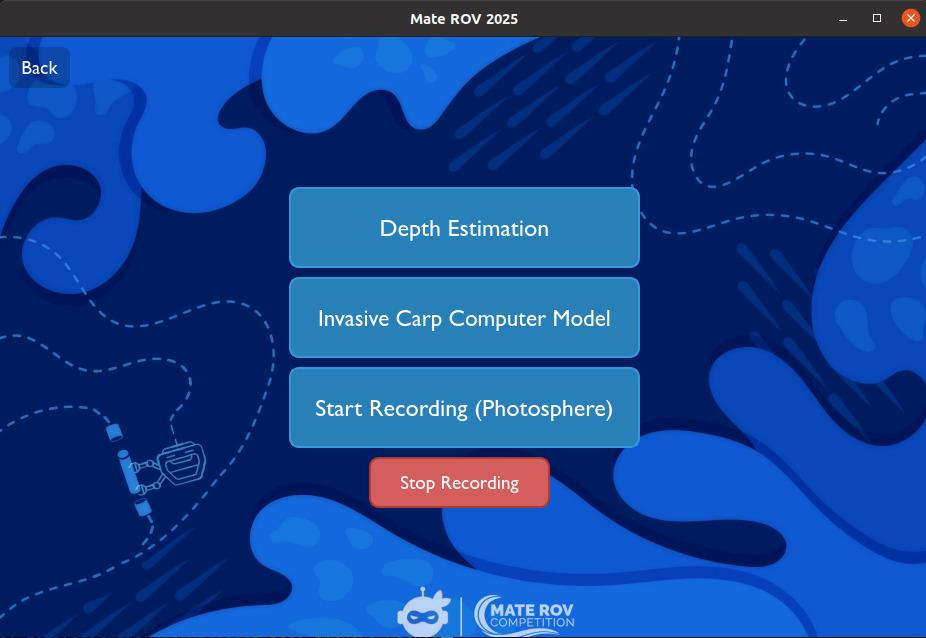
\includegraphics[width=0.8\columnwidth]{Sections/2Design Rationale/images/Engineer_interface.jpeg}
    \caption{Screenshot of the Engineer interface.}
    \label{fig:Engineer_interface}
\end{figure}

\vspace{0.2cm}
\textbf{Float Interface}
The Float interface enables communication with the float before vertical profiling begins and displays depth data along with additional metrics post-profile.

\paragraph{Kinematics}
The Kamikaze's movement underwater may be one of the most important aspects of
the design. We had to ensure stability, maneuverability, and speed. We achieved
this by focusing on two main aspects:
\begin{itemize}
        
    \item \textbf{Thrusters Configuration:} We employed a seventh thruster this year to
        improve the robot's maneuverability as shown in figure \ref{fig:thruster}. With the current vectored thrusters
        configuration and this new thruster, we can achieve motion in 6 degrees of freedom.
        This novel configuration may be the first of its kind to allow for such a wide range of motion while only using 7 thrusters.
        \begin{figure}[h]
            \centering
            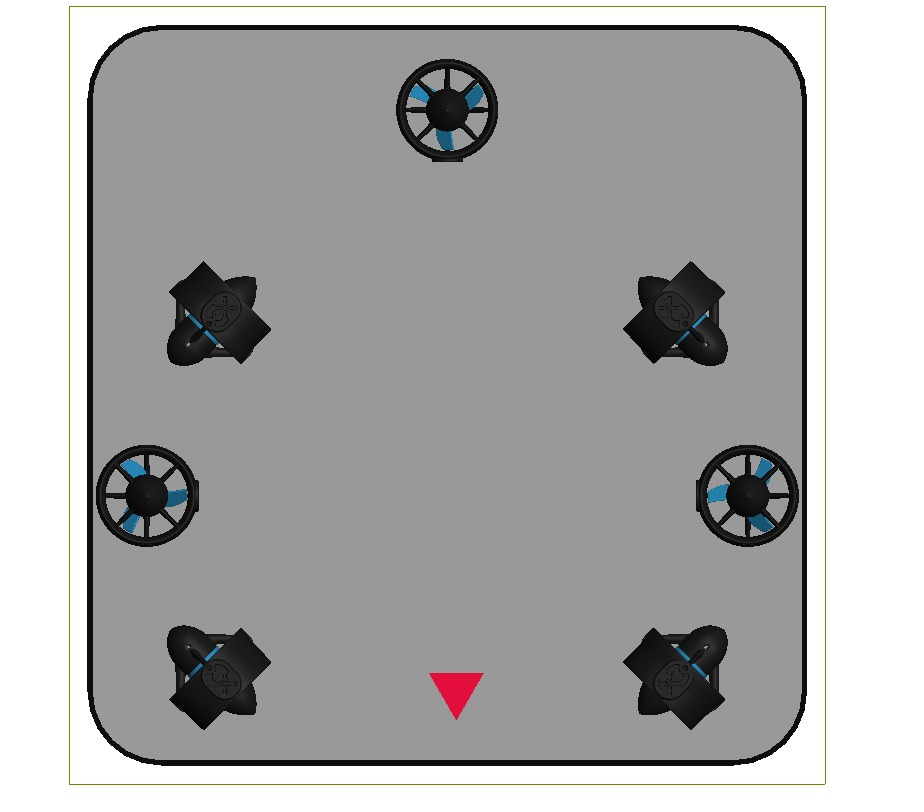
\includegraphics[width=0.3\textwidth]{Sections/2Design Rationale/images/Thrusters.png}
            \caption{Thruster Configuration}
            \label{fig:thruster}
        \end{figure}

        \item \textbf{PID Control:} We have implemented PID controllers for all critical movement axes, allowing for
        precise control over the robot's movement and ensures that it remains stable in the water. We implemented an FFT (Fast Fourier Transform)
        based auto-tuning algorithm to tune the PID parameters, as this is our first year using the new Vehicle. We also supplemented the algorithm with a live
        plotting feature, shown in figure \ref{fig:pid_live},
         to allow for manual adjustments to the PID parameters.
\end{itemize}
\begin{figure}[h]
    \centering
    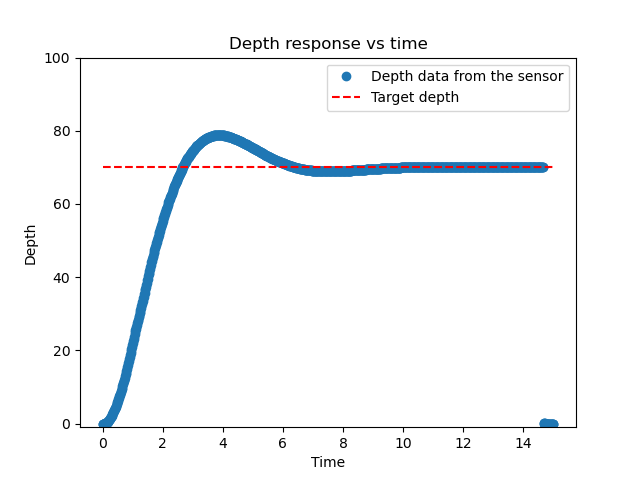
\includegraphics[width=0.5\textwidth]{Sections/2Design Rationale/images/Pid.png}
    \caption{Live Plotting of PID Parameters}
    \label{fig:pid_live}
\end{figure}

\paragraph{Open Sourcing the Kamikaze}
We have all of our working code available on our GitHub repository. A lot of effort
was made this year to maintain, document, and clean up the code, making it easier
for future teams to understand and build upon. We believe that this is a crucial
step in the development of the Kamikaze, as it allows for a more collaborative
environment and ensures that the knowledge gained from each year is not lost. 




\paragraph{Some third point} \ \\
\vspace{-0.5cm}

some software system talk.